% Options for packages loaded elsewhere
\PassOptionsToPackage{unicode}{hyperref}
\PassOptionsToPackage{hyphens}{url}
%
\documentclass[
]{article}
\usepackage{amsmath,amssymb}
\usepackage{lmodern}
\usepackage{ifxetex,ifluatex}
\ifnum 0\ifxetex 1\fi\ifluatex 1\fi=0 % if pdftex
  \usepackage[T1]{fontenc}
  \usepackage[utf8]{inputenc}
  \usepackage{textcomp} % provide euro and other symbols
\else % if luatex or xetex
  \usepackage{unicode-math}
  \defaultfontfeatures{Scale=MatchLowercase}
  \defaultfontfeatures[\rmfamily]{Ligatures=TeX,Scale=1}
\fi
% Use upquote if available, for straight quotes in verbatim environments
\IfFileExists{upquote.sty}{\usepackage{upquote}}{}
\IfFileExists{microtype.sty}{% use microtype if available
  \usepackage[]{microtype}
  \UseMicrotypeSet[protrusion]{basicmath} % disable protrusion for tt fonts
}{}
\makeatletter
\@ifundefined{KOMAClassName}{% if non-KOMA class
  \IfFileExists{parskip.sty}{%
    \usepackage{parskip}
  }{% else
    \setlength{\parindent}{0pt}
    \setlength{\parskip}{6pt plus 2pt minus 1pt}}
}{% if KOMA class
  \KOMAoptions{parskip=half}}
\makeatother
\usepackage{xcolor}
\IfFileExists{xurl.sty}{\usepackage{xurl}}{} % add URL line breaks if available
\IfFileExists{bookmark.sty}{\usepackage{bookmark}}{\usepackage{hyperref}}
\hypersetup{
  pdftitle={Hippocampal subfield},
  pdfauthor={Daniela Cossio},
  hidelinks,
  pdfcreator={LaTeX via pandoc}}
\urlstyle{same} % disable monospaced font for URLs
\usepackage[margin=1in]{geometry}
\usepackage{graphicx}
\makeatletter
\def\maxwidth{\ifdim\Gin@nat@width>\linewidth\linewidth\else\Gin@nat@width\fi}
\def\maxheight{\ifdim\Gin@nat@height>\textheight\textheight\else\Gin@nat@height\fi}
\makeatother
% Scale images if necessary, so that they will not overflow the page
% margins by default, and it is still possible to overwrite the defaults
% using explicit options in \includegraphics[width, height, ...]{}
\setkeys{Gin}{width=\maxwidth,height=\maxheight,keepaspectratio}
% Set default figure placement to htbp
\makeatletter
\def\fps@figure{htbp}
\makeatother
\setlength{\emergencystretch}{3em} % prevent overfull lines
\providecommand{\tightlist}{%
  \setlength{\itemsep}{0pt}\setlength{\parskip}{0pt}}
\setcounter{secnumdepth}{-\maxdimen} % remove section numbering
\usepackage{booktabs}
\usepackage{sectsty} \allsectionsfont{\centering\huge}
\usepackage{sectsty} \subsectionfont{\centering\LARGE}
\usepackage{sectsty} \subsubsectionfont{\centering\Large}
\usepackage{sectsty} \paragraphfont{\large}
\usepackage{sectsty} \subparagraphfont{\normalsize}
\usepackage{titlesec}
\usepackage{lipsum}
\usepackage{booktabs}
\usepackage{longtable}
\usepackage{array}
\usepackage{multirow}
\usepackage{wrapfig}
\usepackage{float}
\usepackage{colortbl}
\usepackage{pdflscape}
\usepackage{tabu}
\usepackage{threeparttable}
\usepackage{threeparttablex}
\usepackage[normalem]{ulem}
\usepackage{makecell}
\usepackage{xcolor}
\ifluatex
  \usepackage{selnolig}  % disable illegal ligatures
\fi

\title{Hippocampal subfield}
\author{Daniela Cossio}
\date{09 September 2024}

\begin{document}
\maketitle

{
\setcounter{tocdepth}{3}
\tableofcontents
}
\newpage

\section{Methods}

\vspace{1cm}
\vspace{1cm}

\section{Results}
\vspace{1cm}
\subsection{Angular Error}
\vspace{1cm}
\vspace{1cm}

\subsubsection{Average}

Total N= 27 F=16 M=11

\paragraph{CA1}

~ There were no significant associations between CA1 and average angular
error across men and women. ( Correlations are not controlled by sex.)
All linear regressions run with a pearson \vspace{1cm}

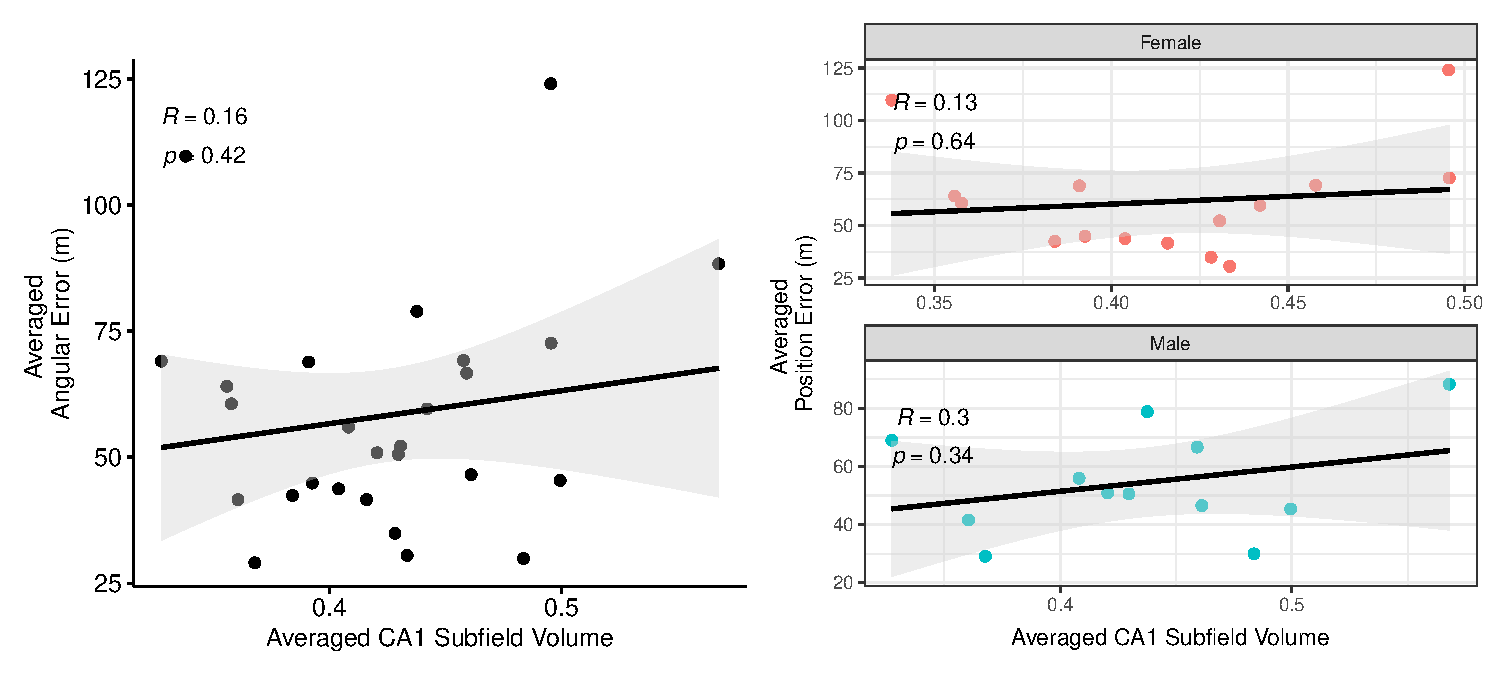
\includegraphics{hippocampal_subfield_files/figure-latex/unnamed-chunk-1-1.pdf}

\newpage
\paragraph{CA2/3}

\subparagraph{There were no significant associations between CA2/3 and average angular error across men and women. The lm was run using a pearson. When conducting the sex stratification, men were analyzed using a spearman and women with a pearson}

~ \vspace{1cm}

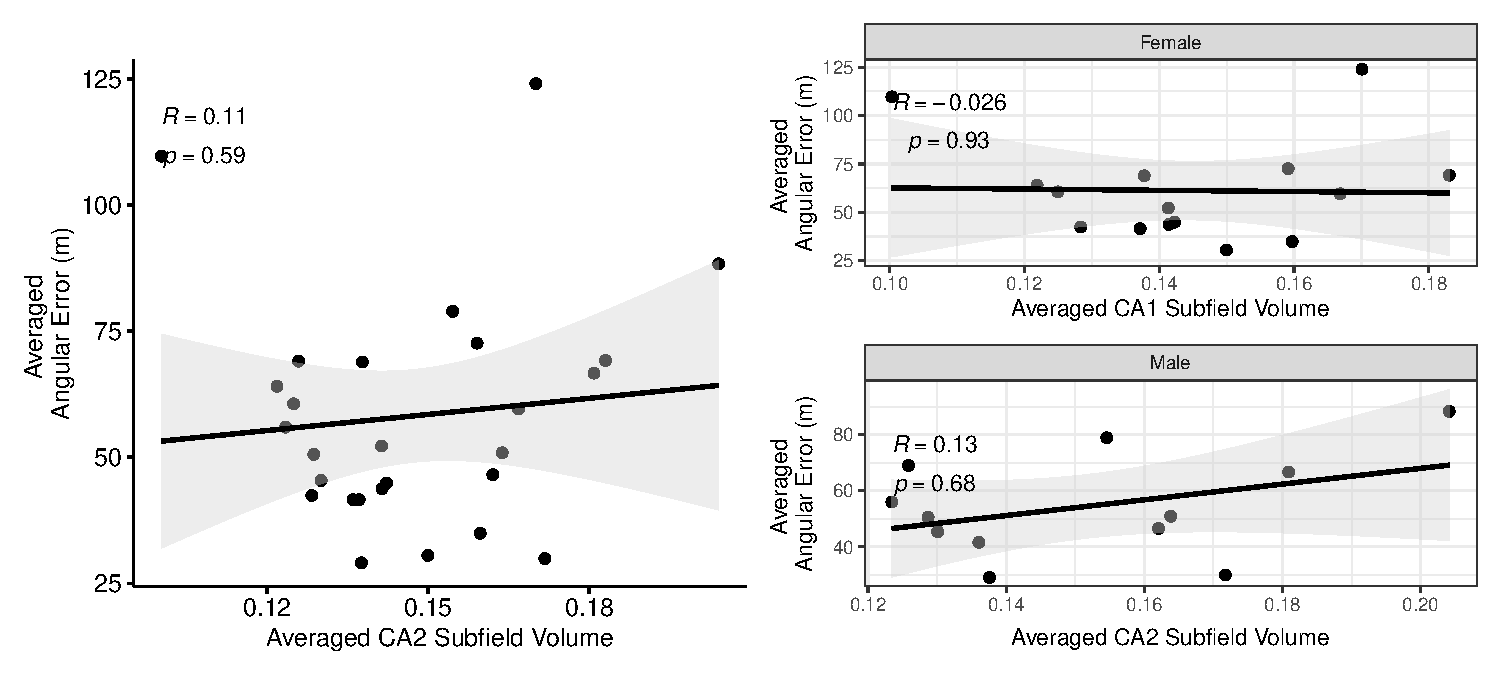
\includegraphics{hippocampal_subfield_files/figure-latex/unnamed-chunk-2-1.pdf}

\paragraph{DG}

~ \vspace{1cm}

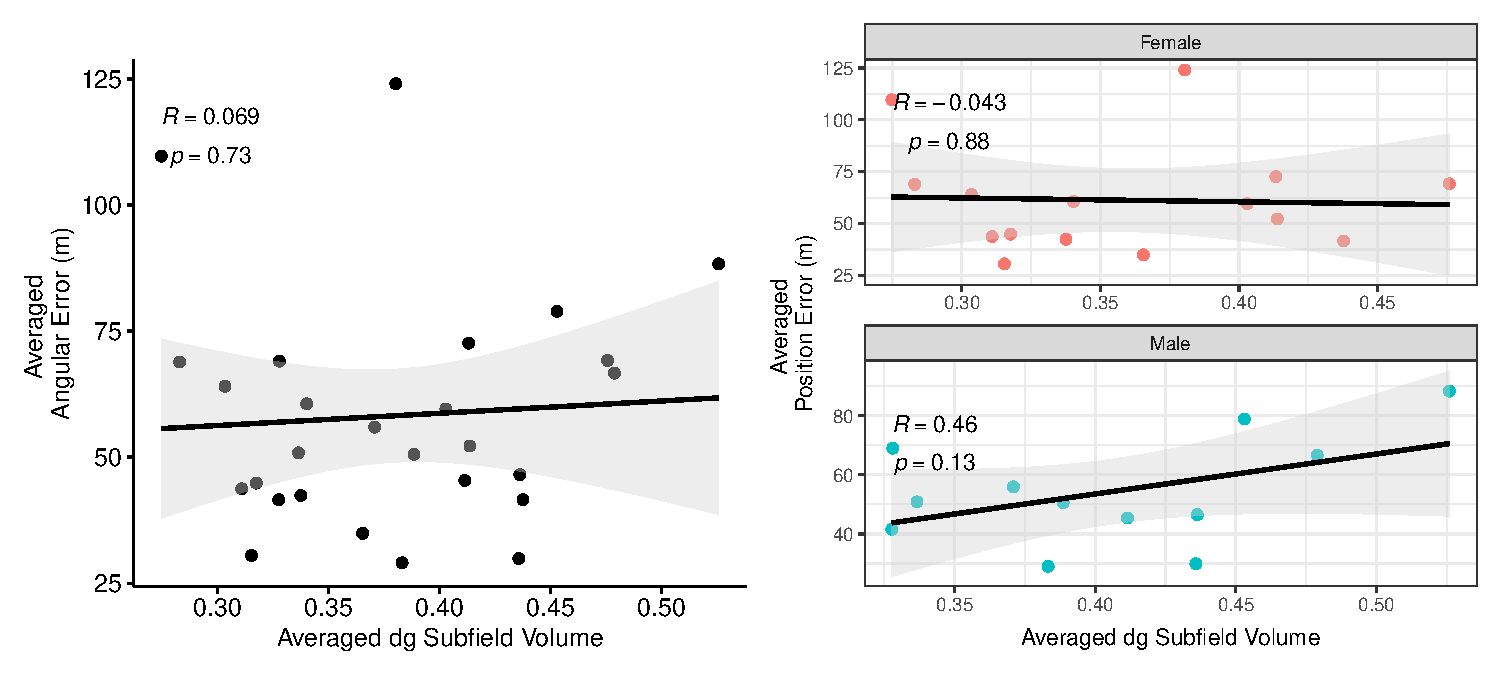
\includegraphics{hippocampal_subfield_files/figure-latex/unnamed-chunk-3-1.pdf}

\newpage
\paragraph{PHC}

~ \vspace{1cm}

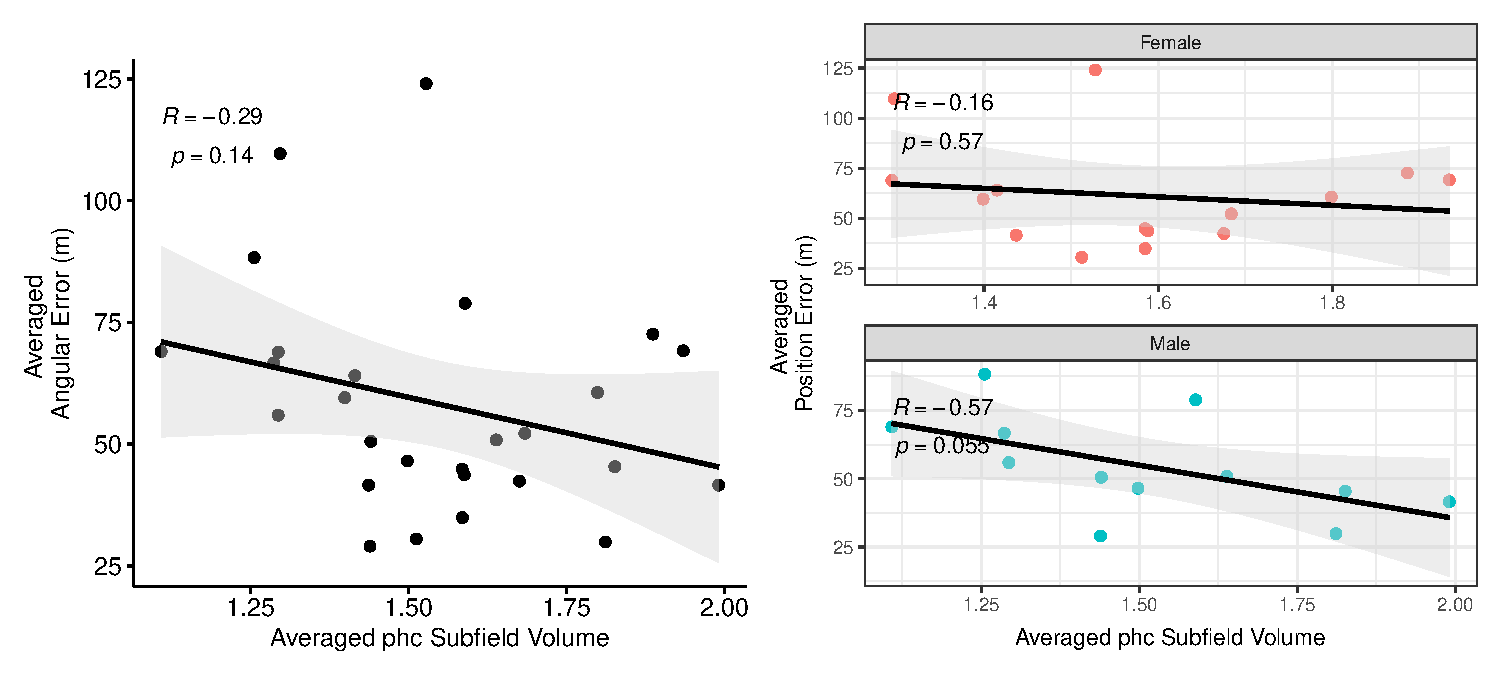
\includegraphics{hippocampal_subfield_files/figure-latex/unnamed-chunk-4-1.pdf}

\paragraph{PRC}

~ \vspace{1cm}

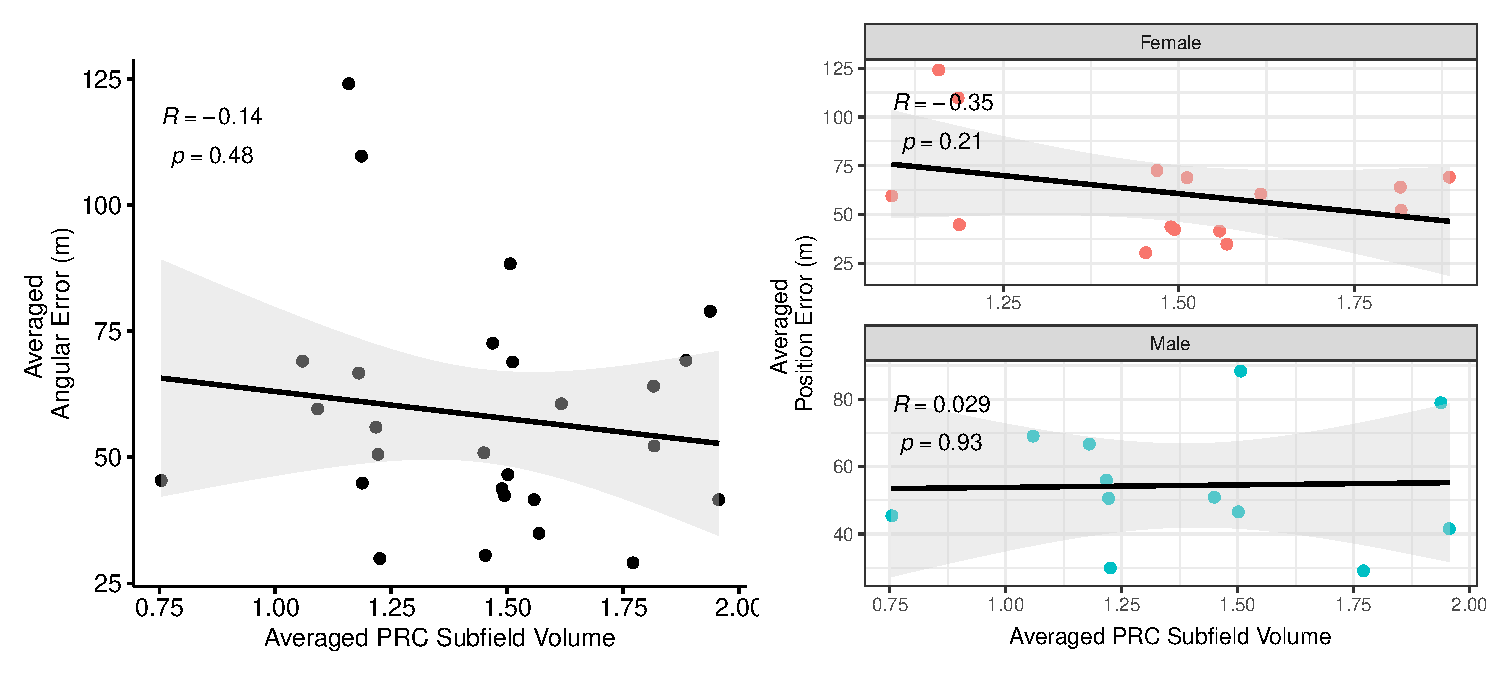
\includegraphics{hippocampal_subfield_files/figure-latex/unnamed-chunk-5-1.pdf}

\newpage
\paragraph{ERC}

~ \vspace{1cm}

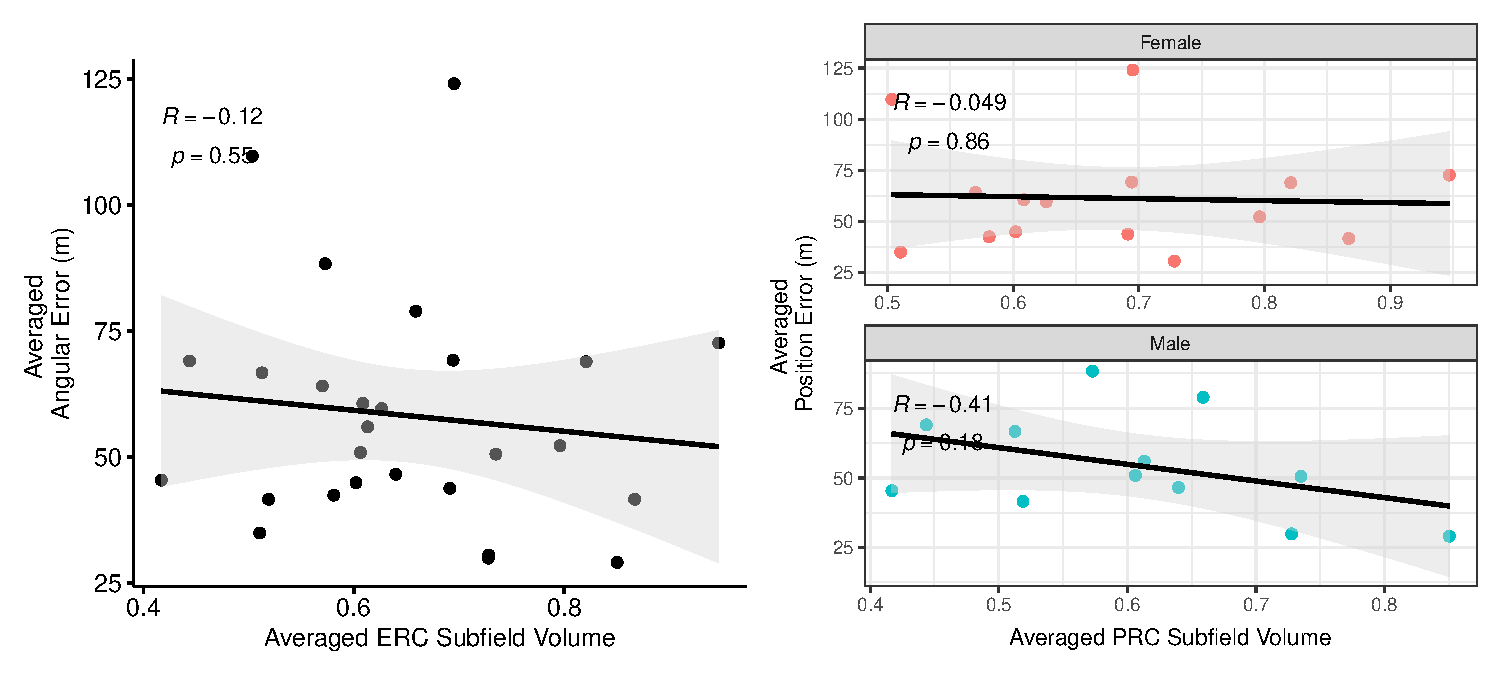
\includegraphics{hippocampal_subfield_files/figure-latex/unnamed-chunk-6-1.pdf}

\paragraph{SUB}

~ \vspace{1cm}

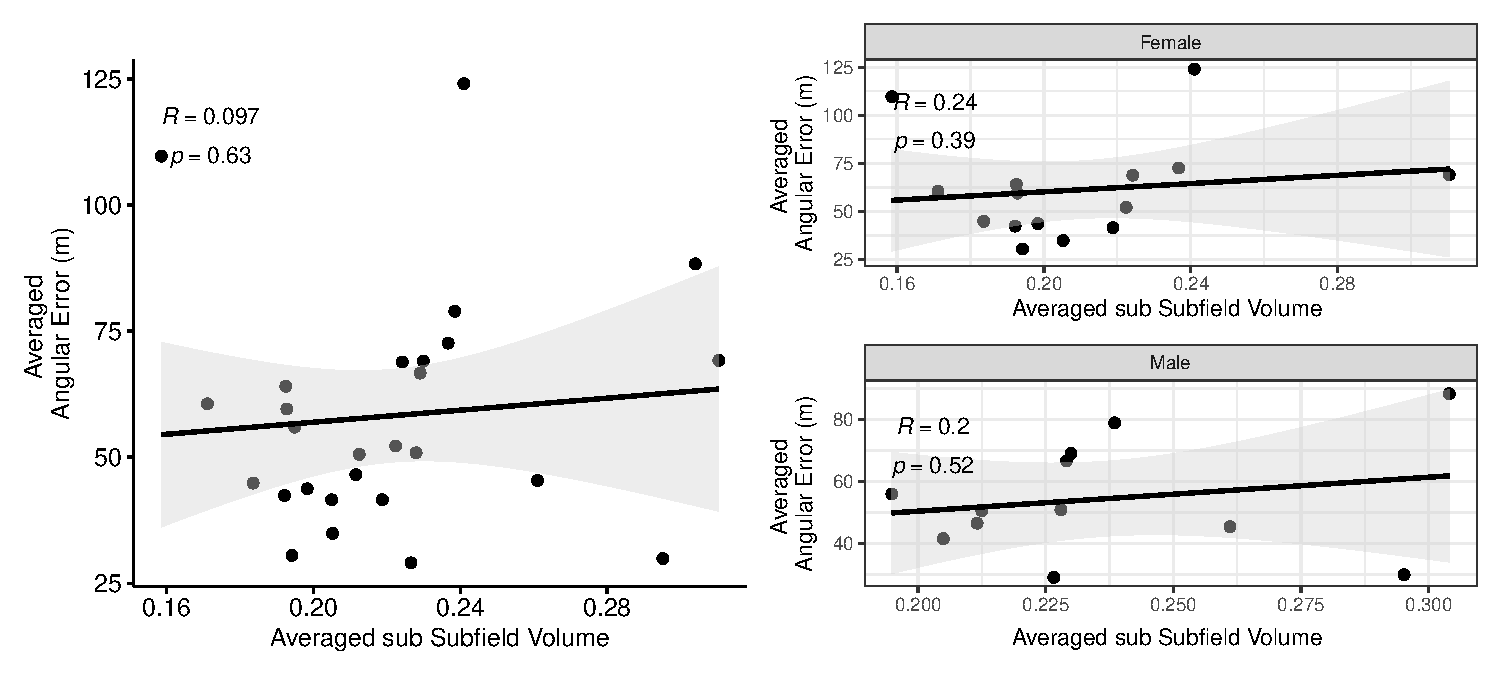
\includegraphics{hippocampal_subfield_files/figure-latex/unnamed-chunk-7-1.pdf}

\newpage
\subsubsection{rad3}

\paragraph{CA1}

~ \vspace{1cm}

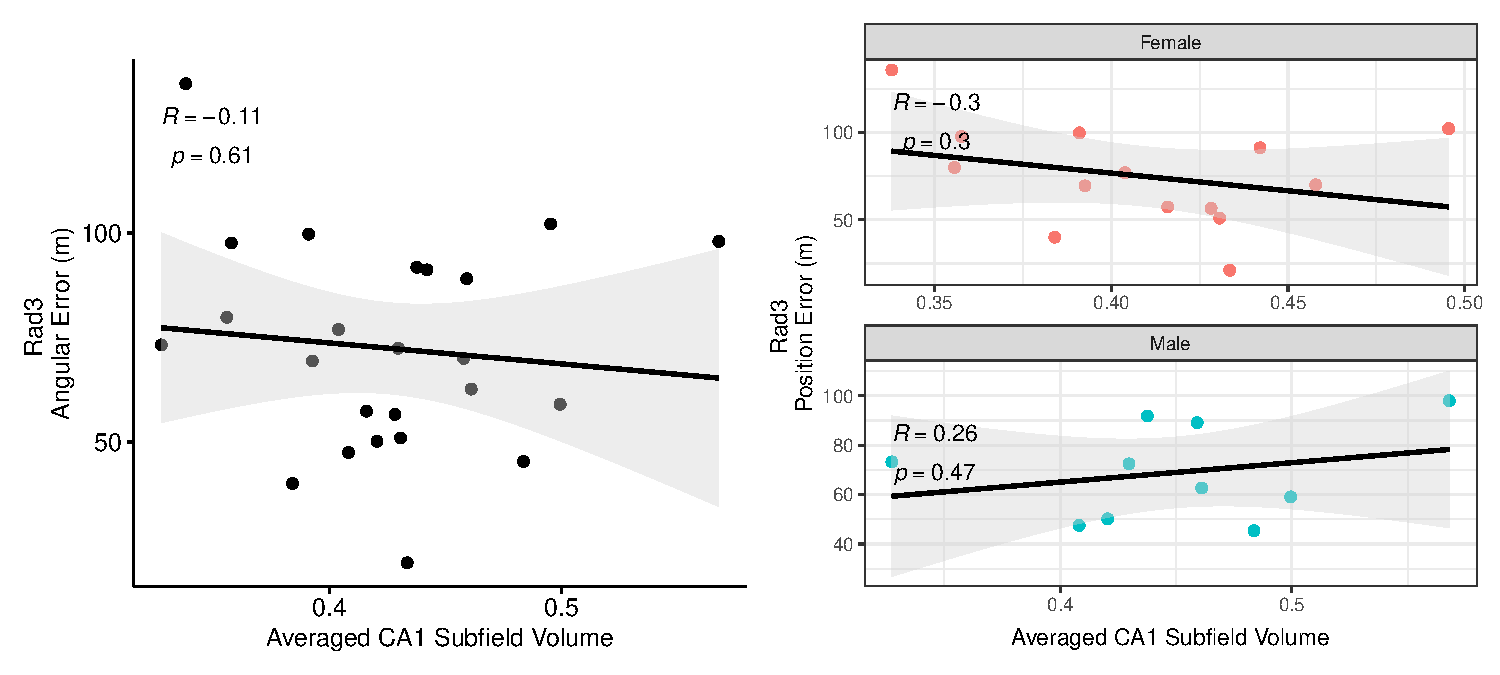
\includegraphics{hippocampal_subfield_files/figure-latex/unnamed-chunk-8-1.pdf}

\newpage
\paragraph{CA2/3}

~ \vspace{1cm}

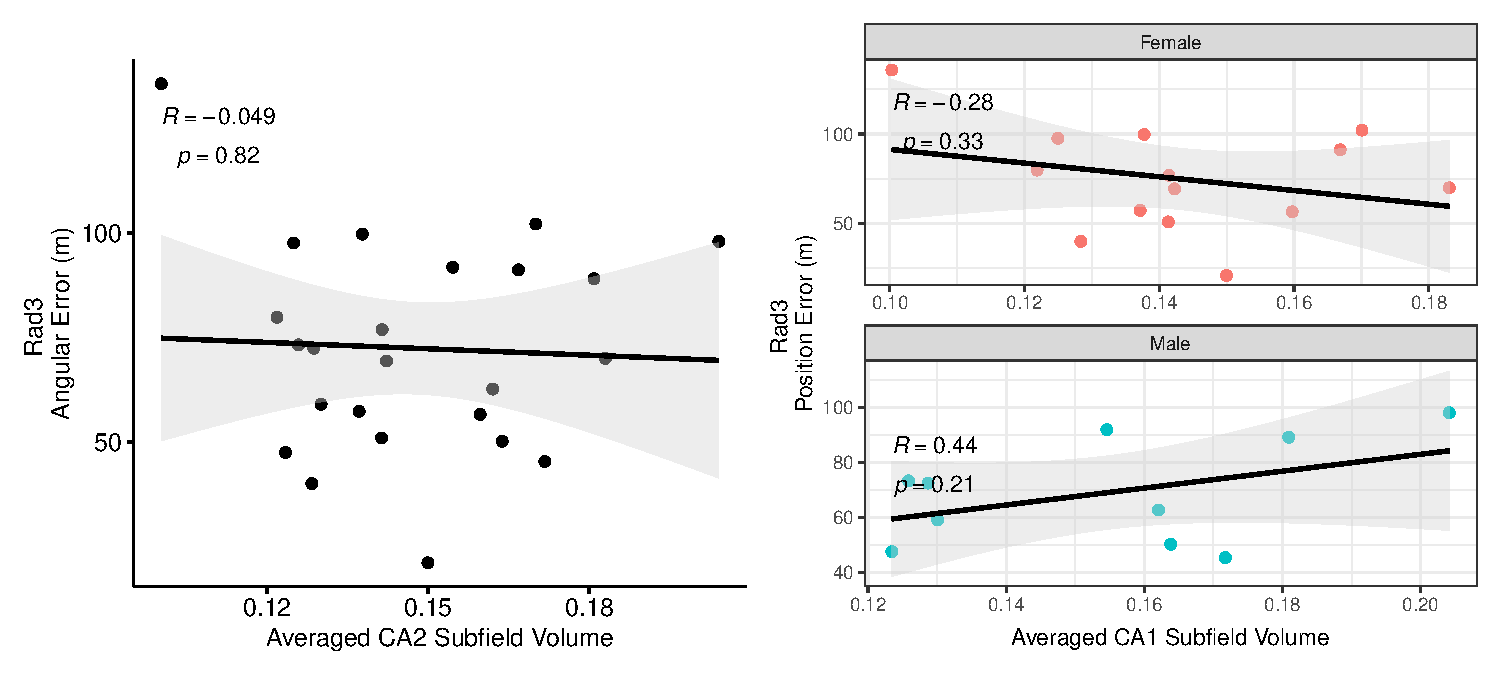
\includegraphics{hippocampal_subfield_files/figure-latex/unnamed-chunk-9-1.pdf}

\paragraph{DG}

~ \vspace{1cm}

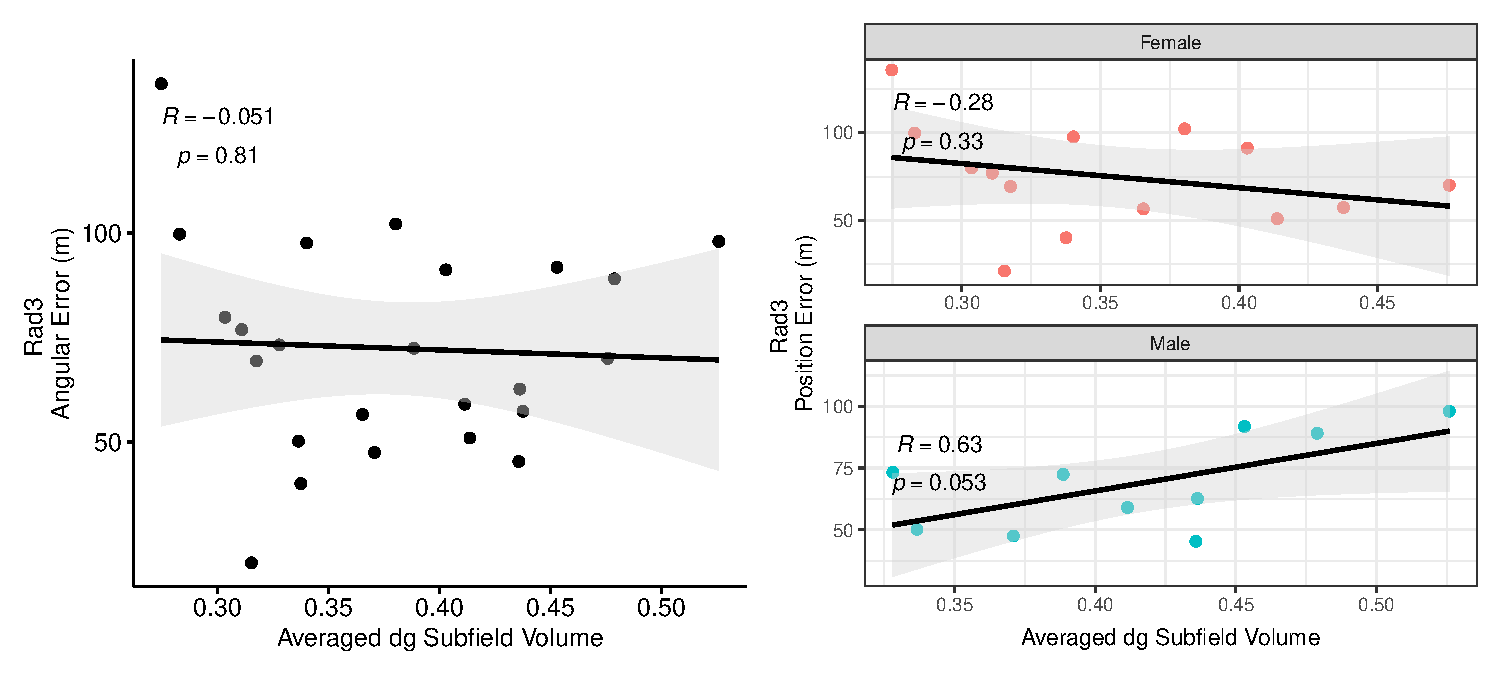
\includegraphics{hippocampal_subfield_files/figure-latex/unnamed-chunk-10-1.pdf}

\newpage
\paragraph{PHC}

~ \vspace{1cm}

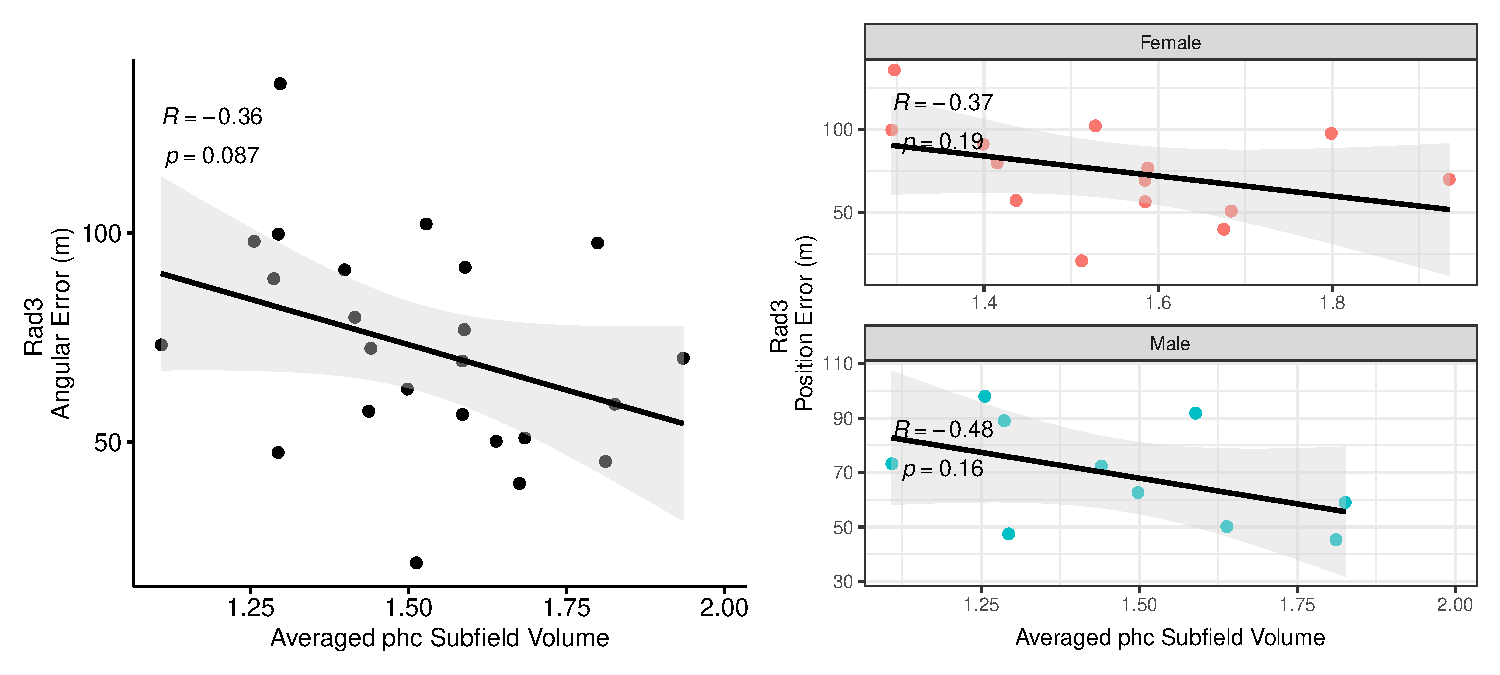
\includegraphics{hippocampal_subfield_files/figure-latex/unnamed-chunk-11-1.pdf}

\paragraph{PRC}

~ \vspace{1cm}

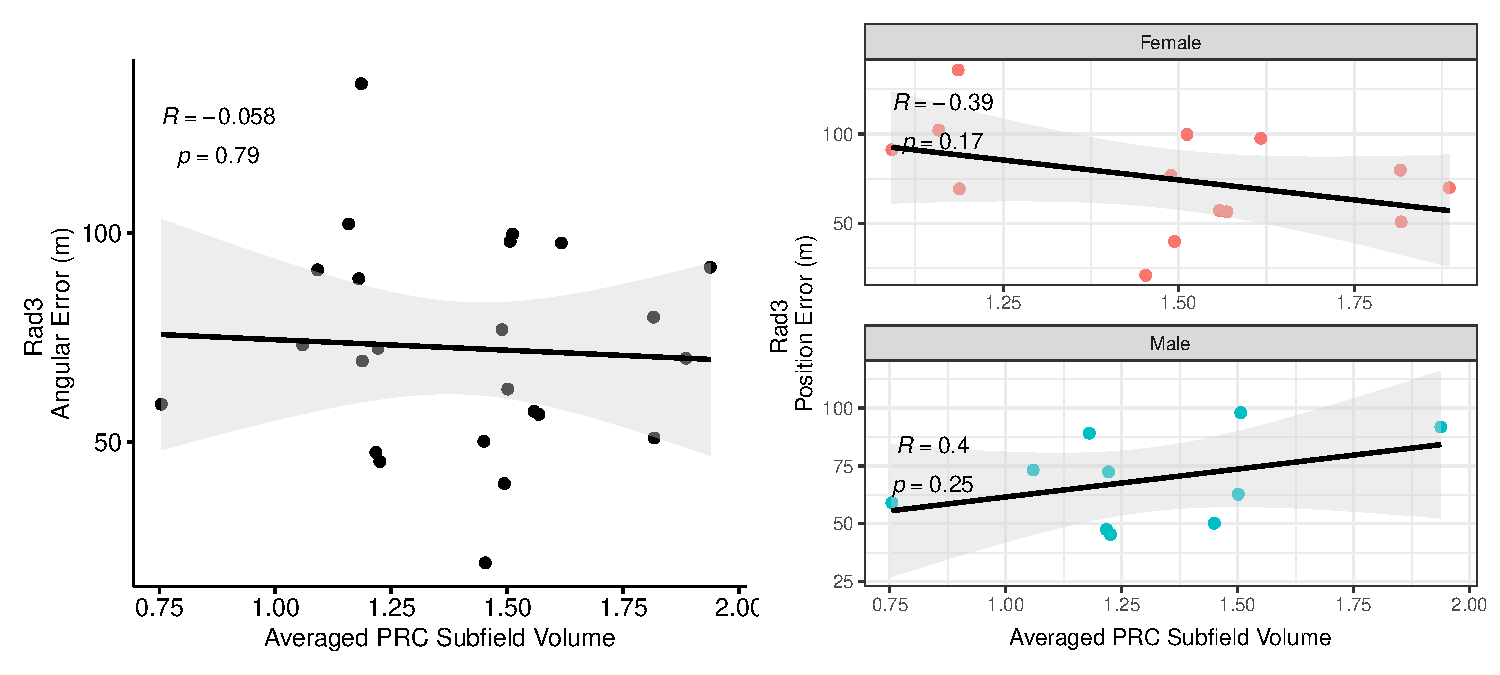
\includegraphics{hippocampal_subfield_files/figure-latex/unnamed-chunk-12-1.pdf}

\newpage
\paragraph{ERC}

~ \vspace{1cm}

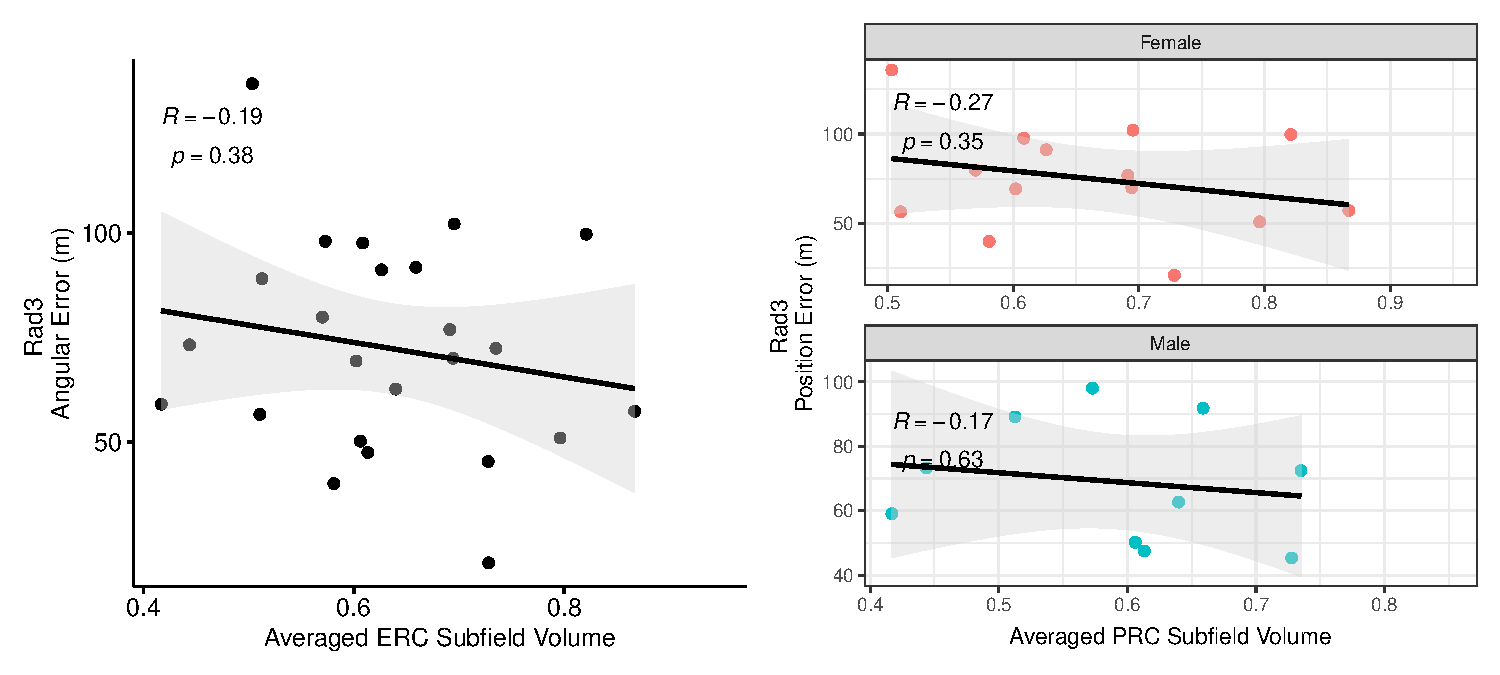
\includegraphics{hippocampal_subfield_files/figure-latex/unnamed-chunk-13-1.pdf}

\paragraph{SUB}

~ \vspace{1cm}

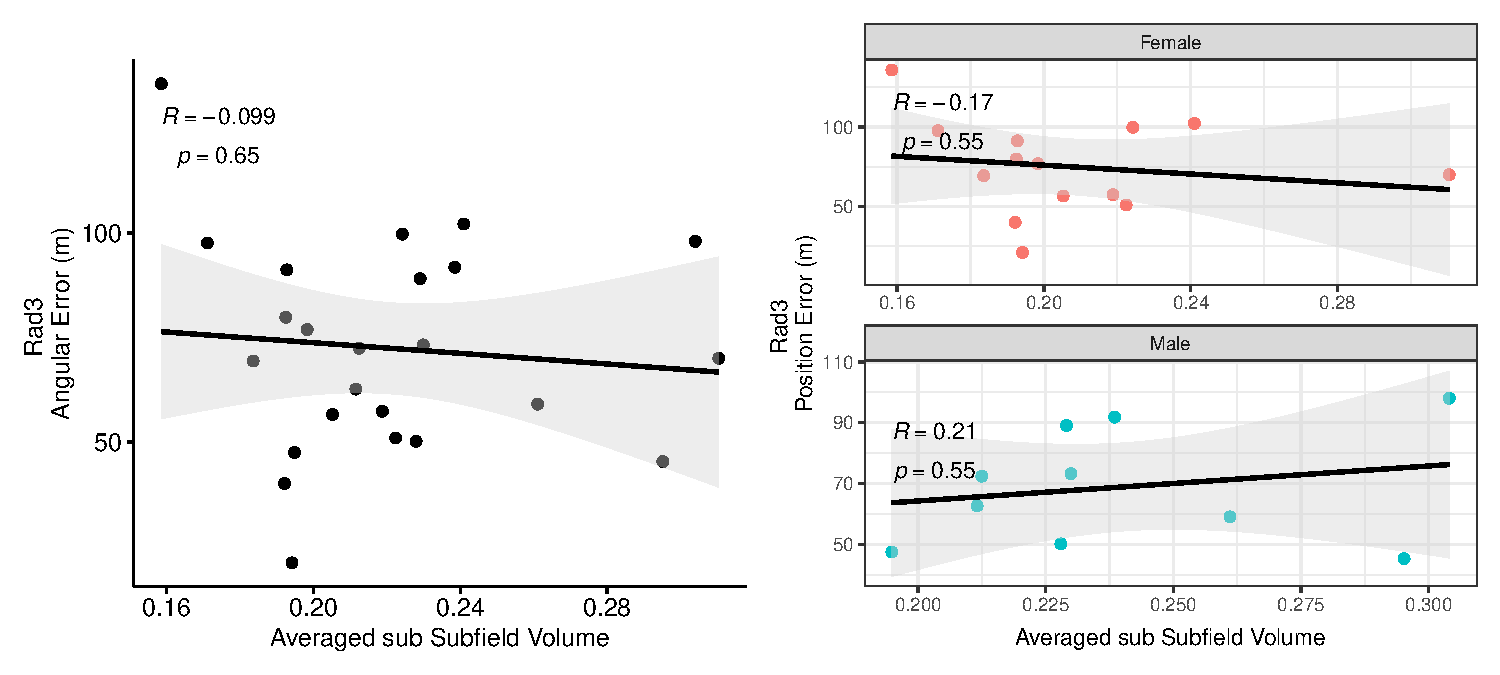
\includegraphics{hippocampal_subfield_files/figure-latex/unnamed-chunk-14-1.pdf}

\end{document}
